%!TeX program=pdflatex
%!TeX encoding=utf8
%!TeX spellcheck = en_US
%!TeX root = ../../messageVortex.tex
\partepigraph{Atoms are very special: they like certain particular partners, certain particular directions, and so on. It is the job of physics to analyze why each one wants what it wants.}{Richard P. Feynman}
\part{Analysis of MessageVortex}
\chapter{Analysis on Common Internet Protocols Suitable as Transport Layers for MessageVortex\label{sec:transportProtocols}}

\section{Introduction}
The following sections list common Internet protocols. We analyze those protocols for the fitness as transport layer of message vortex. 

\section{Methods}

All sections are structured the same way. We first refer to the protocol or standard and describe it in the simplest possible form. We refer to subsequent standards if required to consider extensions where sensible. We then apply the previously referenced criteria and make a concise summary of the suiting of the protocol as a transport layer. The findings of this section is listed in table \ref{tab:protoSuitCrit}. The list here does not reflect the quality or maturity of the protocols. It is a simple analysis of suiting as a transport layer.

All sections are structured the same way. 
\begin{itemize}
	\item Description\\
	We first refer to the protocol or standard and describe it in the simplest possible form. We refer to subsequent standards if required to consider extensions where sensible.
	\item Apply criteria\\\\
	We then apply the previously referenced criteria and make a concise summary of the suiting of the protocol as a transport layer. The findings of this section is listed in table \ref{tab:protoSuitCrit}. The list here does not reflect the quality or maturity of the protocols. It is a simple analysis of suiting as a transport layer.
\end{itemize} 

\subsection{Applied Criteria}
\begin{itemize}
	\item Widely adopted (Ct1)\\
	The more widely adopted and used a protocol is, the harder it is due to the sheer mass for an adversary to monitor , filter, or block the protocol. This is important for censorship resistance of the protocol. 
	\item Reliable (Ct2)\\
	Message transport between peers should be reliable. As messages may arrive anytime from everywhere, we do not have means to synchronize the peer partners on a higher level without investing a considerable effort. Furthermore, the availability of information when what type of information should be available at a specific point in the system would drastically simplify the identification of peers. To avoid synchronization, we do look for inherently reliable protocols.
	\item Symmetrical built (Ct3)\\
	The transport layer should rely on a peer to peer base. All servers implement a generic routing that requires no prior knowledge of all possible targets. This criterion neglects centralized infrastructures. This criterion may be dropped, assuming that the blending layer or a specialized transport overlay is responsible for routing.
\end{itemize}

\subsection{Analyzed Protocols}
We were unable to find a comprehensive list of protocols being used within the Internet and their bandwidth consumption. A weak reference is \cite{zhou2011examining}. This wekaness is founded in the fact that traffic in this report is callified among two critera: Know server or known port. As streaming services consume a considerable part of the Internet bandwidth (acording to the report more than 60\% download). The focus on the report lies on the bandwidth intense figures. However, leavin aside all sources which are strictly one way or dominated by a small number of companies worldwide, the ``top 10'' list of the report shrinks to the two categories ``File sharing'' (Rank 5; 4.2\% download and 30.2\% upload) and ``Messaging'' (Rank 8; 1.6\% download and 8.3\% upload bandwidth). 

In lack of such material we first collected a list of all common Internet messaging protocols (synchronous and asynchronous). We added furthermore some of the most common transfer protocols such as HTTP and FTP and analyzed this list.

\begin{itemize}
	\item Messaging Protocols
	\begin{itemize}
		\item SMTP
		\item CoAP
		\item MQTT
		\item AMQP
		\item XMPP
		\item WAMP
		\item SMS
		\item MMS
	\end{itemize}
	\item Other Protocols
	\begin{itemize}
		\item FTP, SFTP, and FTPS
		\item TFTP
		\item HTTP
	\end{itemize}
\end{itemize}

The following protocols have been discarded as we have considered them as outdated:
\begin{itemize}
	\item MTP\cite{RFC780} (obsoleted by SMTP)
	\item NNTP\cite{RFC3977} (outdated and has only a small usage acording to \cite{kim2010today})
\end{itemize}

We furthermore discarded all RPC-related protocols as they would by definition violate Ct3.

\section{Analysis}
\subsection{HTTP}
The HTTP protocol allows message transfer from and to a server and is specified in RFC2616 \cite{rfc2616}. It is not suitable as a communication protocol for messages due to the lack of notifications. There are some extensions that would allow such communications (such as WebDAV). Still, in general, even those are not suitable as they require a continuous connection to the server to get notifications. Having a ``rollup'' of notifications when connecting is not there by default but could be implemented on top of it. HTTP servers listen on standard ports 80 or 443 for incoming connects. The port 443 is equivalent to the port 80 except for the fact that it has a wrapping encryption layer (usually TLS). The incoming connects (requests) must offer a header part and may contain a body part that would be suitable for transferring messages to the server. The reply to this request is transferred over the same TCP connection containing the same two sections.

HTTP0.9-HTTP/1.1 are clear text protocols which are human-readable (except for the data part which might contain binary data). The HTTP/2\cite{rfc7540} protocol is using the same ports and default behavior. Unlike HTTP/0.9-HTTP/1.1, it is not a clear text but encodes headers and bodies in binary form. 

To be a valid candidate as storage, unauthenticated WebDAV support, as specified in \cite{rfc4918}, must be assumed.

The protocol does satisfy the first two main criteria (Ct1: Widely Adopted and Ct2: Reliable). The main disadvantage in terms of a message transport protocol is that this protocol is not symmetrically. A server is always just ``serving requests'' and not sending information actively to peers. This Request-Reply violates criteria (Ct3: Symmetrically built) and makes the protocol not a primary choice for message transport. 

It is possible to add such behavior to the blending layer using HTTP servers as pure storage. Such a behavior would however be most likely detectable and thus no longer be censorship resistant.

\subsection{FTP}
FTP is defined in RFC959\cite{RFC959}. This Protocol is intended for authenticated file transfer only. There is an account available for general access (``anonymous''). This account does normally not offer upload rights for security reasons. It is possible to use FTP as a message transfer endpoint. The configuration would work as follows: the user ``anonymous'' has upload rights only. It is unable to download or list a directory. A node may upload a message with a random name. In case a collision arises, the node retries with another random name. The blending layer picks messages up using an authenticated user. This workaround has multiple downsides. At first, handling FTP that way is very uncommon and usually requires an own dedicated infrastructure. Such beavior would make the protocol again possibly detectable. Secondly, passwords are always sent in the clear within FTP. Encryption as a wrapping layer (FTPS) is not common, and SFTP (actually a subsystem of SSH) has nothing in common with FTP except for the fact that it may transfer files as well.

Furthermore, FTP may be problematic when used in active mode for firewalls. All these problems make FTP not very suitable as a transport layer protocol. FTPS and SFTP feature similar weaknesses as the FTP version in terms of detectability of non-standard behavior.

Like in HTTP, a disadvantage of FTP in terms of a message transport protocol is that this protocol is not symmetrically. A server is always just ``serving requests'' and not sending information actively to peers. This Request-Reply violates criteria (Ct3: Symmetrically built) and makes the protocol not a primary choice for message transport. The Protocol, however, satisfies the first two criteria  (Ct1: Widely Adopted and Ct2: Reliable).

\subsection{TFTP}
TFTP has, despite its naming similarities to FTP, very little in common with it. TFTP is a UDP based file transfer protocol without any authentication scheme. The possibility of unauthenticated message access makes it not suitable as a transport layer. The protocol is due to the use of UDP in a meshed network with redundant routes. Since the Internet has a lot of these redundant routes, this neglects the use of this protocol.

TFTP is rarely ever used on the Internet, as its UDP based nature is not suitable for a network with redundant routes. Not being common on the Internet violates criterion one (Ct1: Widely Adopted). TFTP is not symmetrically. This means that a server is always just ``serving requests'' and not sending information actively to peers. This Request-Reply violates criteria (Ct3: Symmetrically built) and makes the protocol not a primary choice for message transport. The Protocol furthermore violates Ct2 (Ct2: Reliable) as it is based on UDP without any additional error correction.

\subsection{MQTT}
MQTT is an ISO standard (ISO/IEC PRF 20922:2016) and was formerly called MQ Telemetry Transport. The current standard as the time of writing this document was 3.1.1 \cite{mqtt}. 

The protocol runs by default on the two ports 1883 and 8883 and can be encrypted with TLS. MQTT is a publish/subscribe based message-passing protocol that is mainly targeted to m2m communication. This Protocol requires the receiving party to be subscribed to a central infrastructure in order to be able to receive messages. This makes it very hard to be used in a system without centralistic infrastructure and having no static routes between senders and recipients. 

The protocol does satisfy the second criterion (Ct2: Reliable). It is in the area of end-user (i.e., Internet) not widely adopted, thus violating Criteria 1 (Ct1: Widely Adopted). In terms of decentralization design, the protocol fails as well (Ct3: Symmetrically built).

\subsection{Advanced Message Queuing Protocol (AMQP)}
The Advanced Message Queuing Protocol (AMQP) was initially initiated by numerous exponents based mainly on finance-related industries. The AMQP-Protocol is either used for communication between two message brokers, or between a message broker and a client\cite{amqp}.

It is designed to be interoperable, stable, reliable, and safe. It supports either SASL or TLS secured communication. The use of such a tunnel is controlled by the immediate sender of a message. In its current version 1.0, it does, however, not support a dynamic routing between brokers\cite{amqp}.

Due to the lack of a generic routing capability, this protocol is therefore not suitable for message transport in a generic, global environment.

The protocol satisfies partially the first criterion (Ct1: Widely Adopted) and fully meets the second criterion (Ct2: Reliable). However, the third criterion is violated due to the lack of routing capabilities between message brokers (Ct3: Symmetrically built).

\subsection{Constrained Application Protocol (CoAP)}
The Constrained Application Protocol (CoAP) is a communication Protocol which is primarily destined to m2m communication. It is defined in RFC7252\cite{RFC7252}.  It is defined as a lightweight replacement for HTTP in IoT devices and is based on UDP.

The protocol does partially satisfy the first criteria (Ct1: Widely Adopted). The second criterion (Ct2: Reliable) is only partially fulfilled as it is based on UDP and does only add limited session control on its own.

The main disadvantage in terms of a message transport protocol is that this protocol is not (like HTTP) symmetrically. This means that a server is always just ``serving requests'' and not sending information actively to peers. This Request-Reply violates criteria (Ct3: Symmetrically built) and makes the protocol not a primary choice for message transport. 

\subsection{Web Application Messaging Protocol (WAMP)}
WAMP is a web-sockets based protocol destined to enable M2M communication. Like MQTT, it is publish respectively subscribe oriented. Unlike MQTT, it allows remote procedure calls (RPC).

The WAMP protocol is not widely adopted (Ct1: Widely Adopted), but it is reliable on a per-node base (Ct2: Reliable). Due to its RPC based capability, unlike MQTT, a routing like capability could be implemented. Symmetrical protocol behavior is therefore not available but could be built in relatively easy.

\subsection{XMPP (jabber)}
XMPP (originally named Jabber) is a synchronous message protocol used in the Internet. It is specified in the documents RFC6120\cite{RFC6120}, RFC6121\cite{RFC6120}, RFC3922\cite{RFC3922}, and RFC3923\cite{RFC3923}. The protocol is a very advanced chat protocol featuring numeros levels of security including end-to-end signing and object encryption\cite{RFC3923}. There is also a stream initiation extension for transferring files between endpoints \cite{xep0096}.

It has generic routing capabilities spanning between known and unknown servers. The protocol offers a message retrieval mechanism for offline messages similarily to POP \cite{xep0013}.

The protocol itself seems to be a strong candidate as a transport layer as it is being used actively on the Internet.

\subsection{SMTP}
The SMTP protocol is currently specified in \cite{RFC5321}. It specifies a method to deliver reliably asynchronous mail objects through a specific transport medium (most of the time, the Internet). The document splits a mail object into a mail envelope and its content. The envelope contains the routing information, which is the sender (one) and the recipient (one or more) in 7-Bit ASCII. The envelope may additionally contain optional protocol extension material. 

The content should be in 7-Bit-ASCII (8-Bit ASCII may be requested, but this feature is not widely adopted). It is split into two parts. These parts are the header (which does contain meta-information about the message such as subject, reply address, or a comprehensive list of all recipients), and the body which includes the message itself. All lines of the content must be terminated with a CRLF and must not be longer than 998 characters, excluding CRLF.

The header consists of a collection of header fields. Each of them is built by a header name, a colon, and the data. The exact outline of the header is specified in \cite{RFC5322} and is separated with a blank line from the body. 

\cite{RFC5321} furthermore introduces a simplistic model for SMTP message-based communication. A more comprehensive model is presented in section \nameref{sec:mailTransport} as the proposed model is not sufficient for a detailed end-to-end analysis.

Traditionally the message itself is mime encoded. The MIME messages are mainly specified in \cite{RFC2045} and \cite{RFC2046}. MIME allows to send messages in multiple representations (alternates), and attach additional information (such as possibly inlined images or attached documents). 

SMTP is one of the most common messaging protocols on the Internet (Ct1: Widely Adopted), and it would be devastating for the business of a country if, for censoring reasons, this protocol would be cut off. The protocol is furthermore very reliable as it has built-in support for redundancy and a thorough message design making it relatively easy to diagnose problems (Ct2: Reliable). All SMTP servers usually are capable of routing and receiving messages. Messages going over several servers are common (Ct3: Symmetrically built), so the third criterion may be considered as fulfilled as well.

SMTP is considered a strong candidate as a transport layer.  

\subsection{SMS and MMS}
SMS capability was introduced in the SS7 protocol. This protocol allows the message transfer of messages not bigger than 144 characters. Due to this restriction in size, it is unlikely to be suitable for this type of communication as the keys being required are already sized similarly, leaving no space for Messages or routing information.

The \nth{3} Generation Partnership Project (3GPP) maintains the Multimedia Messaging Service (MMS). This protocol is mainly a mobile protocol based on telephone networks.

Both protocols are not widely adopted within the Internet domain. There are gateways providing bridging functionalities to the SMS/MMS services. However, the protocol itself is insignificant on the Internet itself. 

\subsection{MMS}
This protocol is just like the SMS protocol accessible through the Internet by using gateways but not directly usable within the Internet.

\section{Results}
We have shown that all common M2M protocols failed mainly at Ct3 as there is no need for message routing. In M2M communication contacting foreign machines is not common. Therefore M2M protocolls are typically using static M2M communication over prepared channels. Such behavior is, however unsuitable for a generic messaging protocol.

Pure storage protocols fail at the same criteria as they typically have a defined set of data sources and data sinks, whereas usually at least the data sources are limited in number. This makes those protocols unsuitable again.

We can clearly state that according to the criteria, only a few protocols are suitable. Table \ref{tab:protoSuitCrit2} on page \pageref{tab:protoSuitCrit} shows that only SMTP and XMPP are suitable protocols. Eventually, similar protocols such as HTTP (with WebDAV) or FTP may be usable as well. 

\begin{table}[h]
	\centering\tiny
	\begin{tabular}{|l|l|l|l|}\hline
		\diaghead{\theadfont protocol Criteria}{Protocol}{Criteria} & \thead{Ct1: Widely adopted}     & \thead{Ct2: Reliable} & \thead{Ct3: Symmetrically built}\\\hline
		HTTP     & $\checkmark$            & $\checkmark$        & $\times$\\              
		FTP      & $\checkmark$            & $\checkmark$        & $\times$\\
		TFTP     & $\times$                & $\times$            & $\times$\\
		MQTT     & \textasciitilde         & $\checkmark$        & $\times$\\              
		AMQP     & \textasciitilde         & $\checkmark$        & $\times$\\
		CoAP     & \textasciitilde         & \textasciitilde     & $\times$\\
		WAMP     & $\times$                & $\checkmark$        & \textasciitilde\\
		XMPP     & $\checkmark$            & $\checkmark$        & $\checkmark$\\
		SMTP     & $\checkmark$            & $\checkmark$        & $\checkmark$\\\hline
	\end{tabular}    
	\caption{comparison of protocols in terms of the suitability as transport layer}
	\label{tab:protoSuitCrit2}
\end{table}

The findings of this short analysis suggested that we should use the two protocols, SMTP and XMPP, for our first standardization. We require at least two to prove that the protocol is agnostic to the transport.

\chapter{Analysis of the Core Operations}
\section{Splitting and Merging}
\section{Encryption and Decryption Operations}
\section{Add and Remove Redundancy Operations}\label{sec:analysisReedSolomon}
%%%%%%%%%%%%%%%%%%%%%%%%%%%%%%%
%%% Preplaced float
%%%%%%%%%%%%%%%%%%%%%%%%%%%%%%%
\begin{figure*}[!t]\centering
	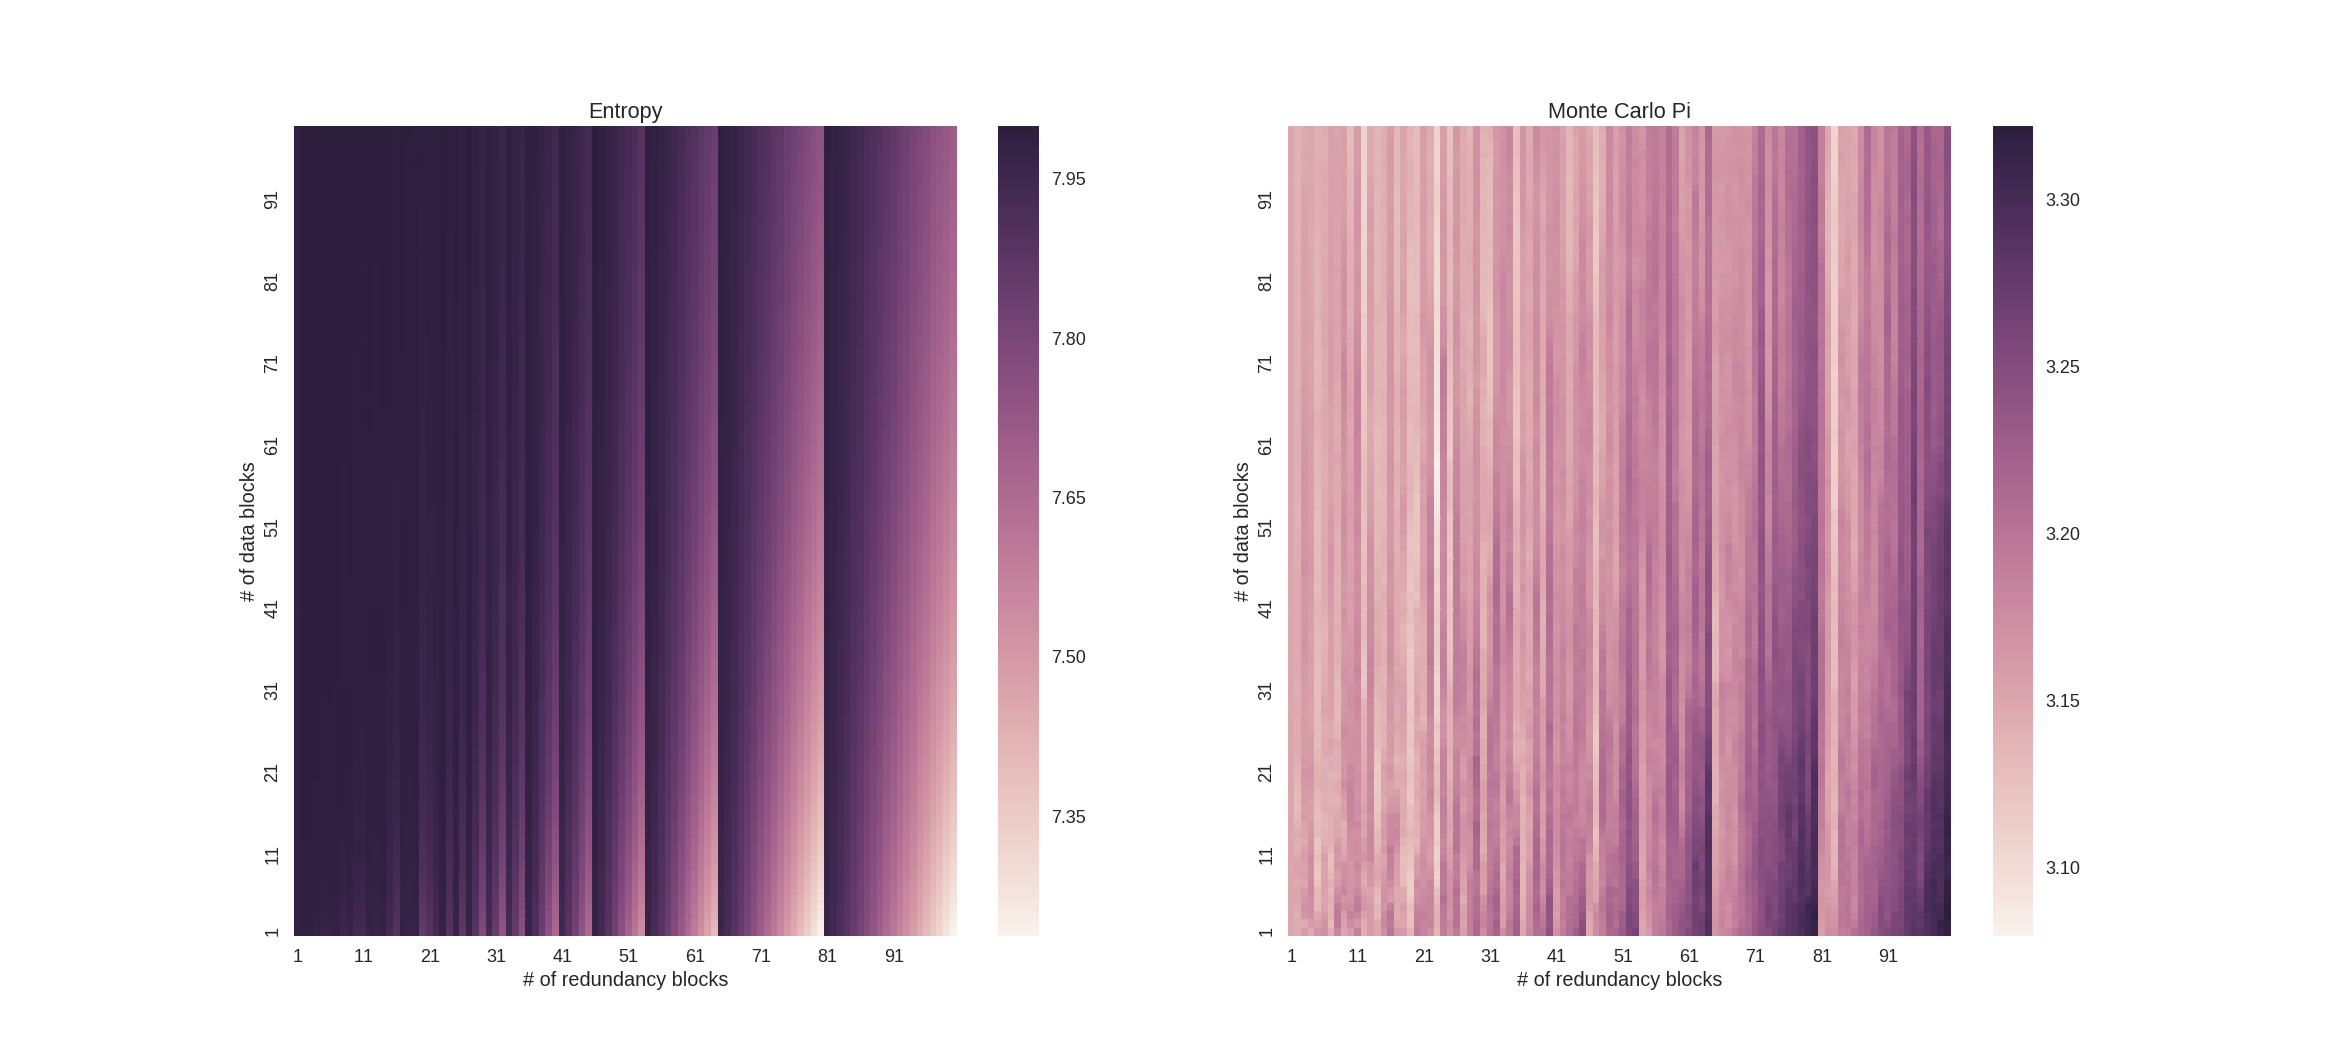
\includegraphics[width=1\textwidth]{inc/randomblock_10kb}
	\caption{Resulting entropy of addRedundancy with and without encryption step}
	\label{fig:entropy}
\end{figure*}


\fxwarning{Fill in results of the RS analysis regarding the findings of the protocol}

\chapter{Well Known Attacks}
In the following sections, we emphasize on possible attacks to an anonymity preserving protocols. These attacks may be used to attack the anonymity of any entity involved in the message channel. In a later stage, we test the protocol for immunity against these classes of attacks.

\section{Broken Encryption Algorithms}
Encryption algorithms may become broken at any time. This either to new findings in attacking them, by more resources being available to an adversary, or by new technologies allowing new kinds of attacks. A proper protocol must be able to react to such threads promptly. This reaction should not rely on a required update of the infrastructure. Users should solely control the grade of security. 

We cannot do a lot for attacks of this kind to happen. However, we might introduce a choice of algorithms, paddings, modes, and key sizes to give the user a choice in the degree of security he wants to have.

We have introduced a way to support a set of independent cryptographic algorithms, paddings ,modes, and prngs. The support of these algorithms does not have to be uniform throughout the system, instead it is sufficient for two neighbouring nodes support the same algoithms in order to be used. 

\section{Attacks Targeting Anonymity}
Attacks targeting users anonymity are the main focus of this work. Many pieces of information may be leaked, and the primary goal should, therefore, rely on the principles established in security.

\begin{itemize}
	\item Prevent an attack\\
	Attack prevention can only be done for attacks that are already known and may not be realistic in all cases. In our protocol, we have strict boundaries defined. A node under attack should at any time of protocol usage (this excepts bandwidth depletion attacks) be able to block malicious identities. Since establishing new identities is costly for an attacker, he should always require far more resources than the defender.
	\item Minimize attack surface\\
	This part of the attack prevention is included by design in the protocol.
	\item Redirect an attack\\
	Although the implementation does not do this, it is possible to handle suspected malicious nodes differently.
	\item Control damage\\
	For us, this means leaving as little information about identities or meta information as possible on untrusted infrastructures. If we leave traces (i.e., message flows, or accounting information) they should have the least possible information content and should expire within a reasonable amount of time.
	\item Discover an attack\\
	The protocol is designed in such a way that attack discovery (such as a query attack) is possible. However, we consider active attacks just as part of the regular message flow. The protocol must mitigate such attacks by design.
	\item Recover from an attack\\
	An attack does always impose a load onto a system's resources regardless of its success. It is vital that a system recovers almost immediately from an attack and is not covered in a non-functional or only partial-functional state either temporarily or permanently.
\end{itemize}

In the following subsections, we list a couple of attack classes that have been used against systems listed in \ref{sec:sysImpl} or the respective academic works. We list the countermeasures which have been taken to deflect these attacks.

\subsubsection{Probing Attacks}
Identifying a node by probing and check their reaction is commonly done when fingerprinting a service. As a node is participating in a network and relaying messages probing may not be evaded. However, it may be made costly for an adversary to do systematic probing. This should be taken into account. Both currently specified transport protocol features an indefinite number of possible accounts. Since not the server but the endpoint address is behaving, node probing is more complicated than in other cases where probing of service is sufficient. 

One of the problems is clear-text requests. These requests may be used on any transport layer account without previous knowledge of any host key. Thus the recommendation in table \ref{tab:protoReplyCrit} is generally not to answer the requests. Routing nodes in jurisdictions not fearing legal repression or prosecution may reply to clear text requests, but it is usually discouraged as they allow harvesting of addresses.

One strategy to avoid would be to put high costs onto clear-text requests in such a way that a clear-text request may have a long reply time (e.g., up to one day). A node is free to blacklist an identity in case of an early reply. This is an insufficient strategy as a big adversary may have lots of identities in stock. Requesting an unusually long key as a plain-text identity does not make sense either as these as well may be kept in stock. We may, however, force a plaintext request to have an identity block with a hash following specific rules. We may, for example, put in a requirement that the first four bytes of the hash of a header block translates to the first four characters of the routing block. At the moment, this has been rejected in the standard for practical reasons. First, as the request is unsolicited, a sender is the only one able to decide the algorithm of the hash. This would allow a requester to choose upon the complexity of the puzzle. Second, any negotiation of the cost of the request would result in the disclosure of the node as VortexNode, which might be unsuitable.

\subsubsection{Hotspot Attacks}
Hotspot attacks aim to isolate high traffic sites within a network. By analyzing specific properties or the general throughput locations with outstanding traffic may be identified. These messages do quite often reveal senders or recipients. Sometimes an intermediate node in an anonymizing system. 

\subsubsection{Message Tagging and Tracing}
When using an anonymization system, a message may be either fully or partially traced or even tagged. Tagging allows one to recognize a message at a later stage and map it to its predecessors. Protocols with tagable messages are not suitable for anonymization systems.

\subsubsection{Side Channel Attacks}
Side-channel attacks are numerous. Especially important to us are attacks related to either lookup in independent channels (e.g., downloading of auxiliary content of a message) or behavior related to timing patterns.

\subsubsection{Sizing Attacks}
There are two kinds of sizing attacks identified to be relevant for us. One is the possibility for matching messages with related sizes, and the other one is to relate message size to the original messages. Both attacks may be considered as a tracing attack and will be analyzed accordingly.

\subsubsection{Bugging Attacks}
Numerous attacks are available through the bugging of a protocol. In this chapter, we outline some of the possibilities and how they may be countered:

\begin{itemize}
	\item Bugging through certificate or identity lookup:\\
	Almost all kinds of proof of identities, such as certificates, offer some revocation facility. While this is a perfect desirable property of these infrastructures, they offer a flaw. Since the location of this revocation information is typically embedded in the proof of identity, an evil attacker might use a falsified proof of identity with a recording revocation point.
	
	There are multiple possibilities to counter such an attack. The easiest one is to do no verification at all. Having no verification is, however, not desirable from the security point of view. Another possibility is only to verify trusted proof of identities. By doing so, the only attacker could be someone having access to a trusted source of proof of identities. A third possibility is to relay the request to another host either by using an anonymity structure such as Tor or by using its infrastructure. Using Tor would violate the ``Zero Trust'' goal. Such a measure would only conceal the source of the verification. It would not hide the fact that the message is processed. A fourth and most promising technology would be to force the sender of the certificate to include a ``proof of non-revocation''. Such a proof could be a timestamped and signed partial CRL. It would allow a node to verify the validity of a certificate without being forced to disclose itself by doing a verification. On the downside has to be mentioned that including proof of non-revocation involves the requirement to accept a certain amount of caching time to be accepted. This allowed caching time reduces the value of the proof as it may be expired in the meantime. It is recommended to keep the maximum cache time as low as 1d to avoid that revoked certificates may be used. 
	
	\item Bugging through DNS traffic:\\
	A standard protocol on the Internet is DNS. Almost all network-related programs use it without thinking. Typically the use of such protocol is only a minor issue since the resolution of a lookup usually done by an ISP. In the case of a small Internet service provider (ISP), this might, however, already become a problem.
	
	The bugging in general attack works as follows: We include a unique DNS name to be resolved by a recipient. This can be done most easily by adding an external resource such as an image. A recipient will process this resource and might, therefore, deliver information about the frequency of reading, or the type of client. 
	
	It must be taken into account that the transport layer will always do DNS lookups and that we may not avoid this attack completely. We may, however, minimize the possibilities of this attack.
	
	\item Bugging through external resources:\\
	A straightforward attack is always to include external resources into a message and wait until they are fetched. In order to avoid this kind of attack, plain text or other self-contained formats should be used when sending a message. As we may not govern the type of contained message, we can make at least recommendations concerning its structure.
\end{itemize}

\subsection{Denial of Service Attacks}
\subsubsection{Censorship}
Whereas traditional censorship is widely regarded as selective information filtering and alteration, very repressive censorship can even include denial of information flows in general. Any anonymity system not offering the possibility to hide in legitimate information flows, therefore not censorship-resistant.

\subsubsection{Denial of service}
An adversary may flood the system in two ways.
\begin{itemize}
	\item He may flood the transport layer exhausting resources of the transport system.\\
	This is a straightforward attack. MessageVortex has no control over the existing transport protocol. Therefore, all flooding attacks on that layer are still effective. However, If an adversary attacks a node, the redundancy of a message may still be sufficient. On the other hand, flooding disrupts at least all other services using the same transport layer on that node. This result may be unacceptable for an attacker. More likely would be censorship.
	\item He may flood the routing layer with invalid messages.\\ 
	Identifying the messages is relatively easy for a node. Usually, it should be sufficient to decode the CPREFIX block of a message. If the CPREFIX is valid, then the header block either identifies a valid identity or processing may be aborted. 
	\item He may flood an accounting layer with newIdentity.\\
	Flooding an accounting layer with identities is possible. Since the accounting layer is capable of adapting costs to a new identity, it may counter this attack by giving large puzzles to new identities. This affects all new identities and not only those flooding. If a flooding attack is carried out over a long time, a node may decide to split its identity. All recent active users get a new identity, whereas the old one opposes high costs. This would force an attacker to work in intervals and is no longer able to make a permanent DoS attack.
\end{itemize}

\subsubsection{Credibility Attack}
Another type of DoS attack is the credibility attack. While not a technical attack, it is very effective. A system not having a sufficiently big user base is offering thus a lousy level of anonymity because the anonymity set is too small or the traffic concealing message flow is insufficient. 

Another way is to attack the reputation of a system in such a way that the system is no longer used. An adversary has many options to achieve such a reduction in credibility. Examples:
\begin{itemize}
	\item Disrupt functionality of a system.\\ 
	This may be done by blocking of the messaging protocol it uses or by blocking messages. Furthermore, an adversary reduces functionality when removing known participants from the network either by law or by threatening.
	\item Publicly dispute the effectiveness of a system.\\
	Disputing the effectiveness is a very effective way to destroy a system. People are not willing to use a system which believed to be compromised if the primary goal of using the system is avoiding being observed.
	\item Reduce the effectiveness of a system.\\
	A system may be considerably loaded by an adversary to decrease the positive reception of the system. He may further use the system to send \defref{UBM} to reduce the overall experience when using the system. Another way of reducing effectiveness is to misuse the system for evil purposes such as blackmailing and making them public.
	\item Dispute the credibility of the system founders.\\
	Another way of reducing the credibility of a system is to undermine its creators. If -- for example -- people believe that a founders' interest was to create a honey pot (e.g., because he is working for a potential state-sponsored adversary) for personal secrets, they will not be willing to use it.
	\item Dispute the credibility of the infrastructure.\\
	If the infrastructure is known or suspected to be run by a potential adversary, people's willingness to believe in such a system is expected to be drastically reduced.
\end{itemize}


\chapter{Identification of Possible Attack Schemes and Mitigation\label{sec:attacks}}
\fxwarning{complete section}
\section{Static Attacks}
\fxwarning{complete section}
\subsection{Bugging and Tagging Attacks}
\fxwarning{complete section}
\subsection{Information Leaking related to Information Available to Routing Nodes}
\fxwarning{complete section}
\subsection{Identification of involved Nodes}
\fxwarning{complete section}
\subsection{Identification of MessageVortex Traffic}
\fxwarning{complete section}
\section{Dynamic Attacks}
\fxwarning{complete section}
\subsection{Attacks against the vortex system itself}
\subsubsection{DoS Attacks against the Transport System}
\subsubsection{DoS by Traffic Replay}
\subsubsection{DoS by Traffic generation}
\subsection{Attacking a single ephemeral Identity of a MessageVortex Node}
\fxwarning{complete section}
\subsubsection{Denial of Service by Exhausting Quotas or Limits}
\subsection{Attacking Sending and Receiving Identities of the MessageVortex System}
\fxwarning{complete section}
\subsubsection{Traffic Highlighting or Traffic Analysis}
\subsection{Recovery of Previously Carried Out Operations}
\fxwarning{complete section}

\fxwarning{complete section}
\chapter{Analysis of the effectiveness of Attack Schemes}
\fxwarning{complete section}
\chapter{Analysis of the Degree of Anonymization in Comparison to other Systems}
\fxwarning{complete section}

